The \gls{pppn} balances protecting the investment against taking part in the movements of the stock.
At maturity on January 15, 2027, the investor is guaranteed to get back 90\% of the invested capital.
On top of that, the note pays a premium if \gls{jpm} ends up outside a corridor around today's price $S_0$ (see Fig.~\ref{fig:jpm-corridors}).
The premium grows with the distance from the corridor, so large moves are rewarded in either direction.

\gls{jpm} is a good fit for such a product.
Over the past year, the stock rose from \$239.56 on November 12, 2024, to \$320.41 at $t=0$, an increase of about 34\%.
Moves of this size are exactly what the premium pays for, while the investor never risks more than 10\% of the capital.

\subsection{Payoff}
The payoff of the \gls{pppn} has two parts: a protected base and a premium that depends on the stock price $S_T$ at maturity.

\paragraph{Principal Protection}
To secure 90\% of the invested amount $N$, part of the capital is invested in a zero-coupon bond.
Its present value is $0.9N e^{-rT}$, and it grows to $0.9N$ at maturity, whatever happens to the stock.

\paragraph{Premium}
Two strikes $K_1 < S_0 < K_2$ define a corridor in which no premium is paid.
Outside the corridor, the premium is proportional to how far the stock has moved:
\begin{equation}
\nonumber
    \begin{aligned}
        \text{Premium}(S_T) =
        \begin{cases}
        \frac{N}{S_0}(K_1 - S_T), & \text{if } S_T < K_1,\\[6pt]
        0, & \text{if } K_1 \leq S_T \leq K_2,\\[6pt]
        \frac{N}{S_0}(S_T - K_2), & \text{if } S_T > K_2.
        \end{cases}
    \end{aligned}
    \qquad\qquad
    \vcenter{\hbox{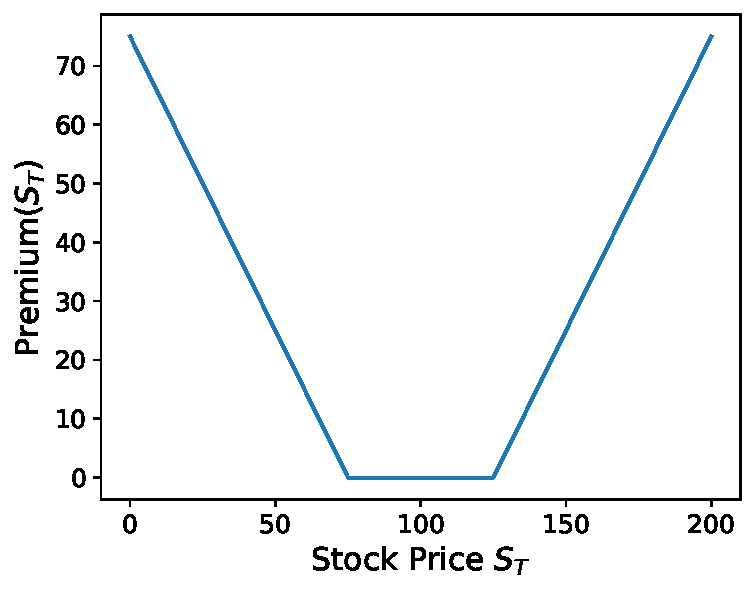
\includegraphics[width=5cm, height=4cm]{pppn_premium_payoff.pdf}}}
\end{equation}
The plot on the right shows an example with $S_0 = 100$, $K_1 = 75$ and $K_2 = 125$.
For the rest of this section, we set $N = S_0$, so that $\frac{N}{S_0} = 1$.

\subsection{Replication}
The bond provides the capital protection.
The premium is replicated by buying $\frac{N}{S_0}$ European puts with strike $K_1$ and $\frac{N}{S_0}$ European calls with strike $K_2$, both with maturity $T$.

\paragraph{Replication Cost}
The issuer also charges a margin $M$ to cover its profit and hedging costs.
We express it as a fraction $m$ of the investment, $M = mN$.
At $t = 0$, the bond, the options and the margin must add up to the amount invested:
\begin{align}
\label{eq-pppn-replication-cost}
    N = 0.9N e^{-rT} + \frac{N}{S_0}\big[EP(K_1, T) + EC(K_2, T)\big] + mN.
\end{align}

\paragraph{Choosing $K_1$ and $K_2$}
Rearranging \eqref{eq-pppn-replication-cost} gives the budget available for the two options:
\begin{align}
    EP(K_1, T) + EC(K_2, T) = S_0 \left( 1 - 0.9e^{-rT} - m \right).
    \label{eq-option-cost}
\end{align}
Strikes are only quoted in steps of 5 or 10, so this equality can usually not be met exactly.
We therefore only require the left-hand side to be at most the budget; any amount left over goes to the issuer.
Fig.~\ref{fig:valid-strike-pairs} shows all strike pairs $(K_1, K_2)$ that satisfy this condition for margins of $0.1\%$, $0.5\%$ and $1.0\%$.
Options with strikes close to $S_0$ are more expensive, because a narrow corridor makes a premium more likely.
A higher margin leaves less money for the options and therefore forces a wider corridor.

\begin{figure}
    \centering
    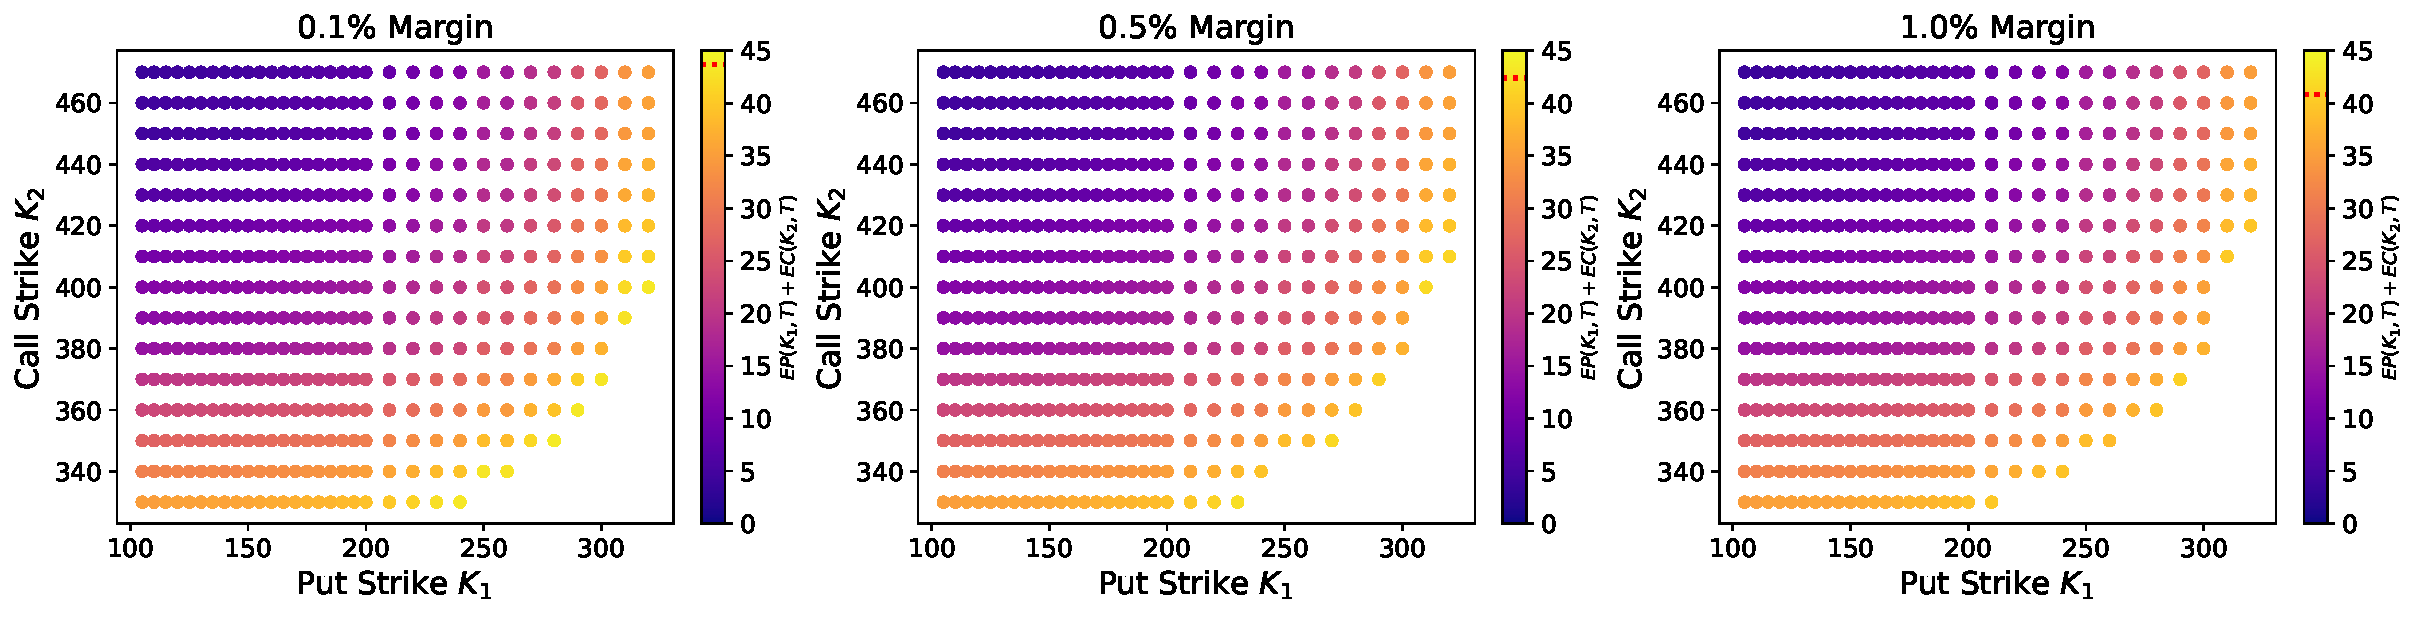
\includegraphics[width=\linewidth]{pppn_valid_strikes.pdf}
    \caption{\textbf{Valid Strike Pairs.} Strike pairs $(K_1, K_2)$ whose combined option cost fits within the budget \eqref{eq-option-cost} for margins of $0.1\%$, $0.5\%$ and $1.0\%$. The colour gives the total cost of both options, and the dotted red line in each colour bar marks the budget.}
    \label{fig:valid-strike-pairs}
\end{figure}

We choose a margin of $m = 0.5\%$, which leaves the issuer a reasonable profit while keeping the product attractive.
With $S_0 = 320.41$, $r = 3.635\%$ and $T = 1.167$, the option budget is $42.41$.
For the investor, the best strikes are those with the narrowest corridor $K_2 - K_1$.
The narrowest valid corridor has a width of 80, and among the pairs that reach it we take the one that uses most of the budget:
\begin{align}
    \nonumber
    EP(270, T) + EC(350, T) = 15.45 + 26.09 = \mathbf{41.54 \leq 42.41}.
\end{align}
The note therefore uses $K_1 = 270$ and $K_2 = 350$.
Fig.~\ref{fig:jpm-corridors} places this corridor on the price history of \gls{jpm}.

\begin{figure}[H]
    \centering
    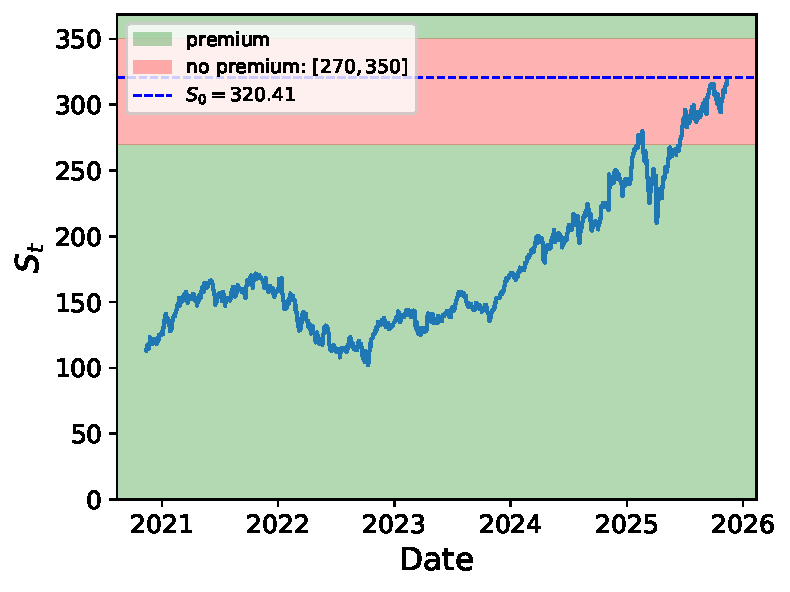
\includegraphics[width=0.5\linewidth]{pppn_jpm_corridors.pdf}
    \caption{\textbf{PPPN Corridor for JPM.} Closing prices of \gls{jpm} over the past five years together with the premium zones of the note. A premium is paid below $K_1 = 270$ and above $K_2 = 350$ (green), but not in between (red).}
    \label{fig:jpm-corridors}
\end{figure}

\subsection{Simulation}
\label{sec-pppn-simulation}
To estimate how the note might perform, we simulate \gls{jpm} as a geometric Brownian motion, discretised with the Euler--Maruyama scheme over the 294 trading days until maturity.
The drift $\mu = 23.47\%$ is the average daily log-return of \gls{jpm} over the past five years, annualised.
The volatility $\sigma = 28.9\%$ is the implied volatility of the options around the chosen strikes\footnote{\url{https://optioncharts.io/options/JPM/volatility-skew?option_type=all&expiration_dates=2027-01-15:m&strike_range=270,350}}.
The options are priced under the risk-neutral measure, but the simulation uses the real-world drift because we want to know how the product is likely to perform.
Further details are given in Appendix~\ref{appendix-monte-carlo-simulation}.

\begin{figure}[H]
    \centering
    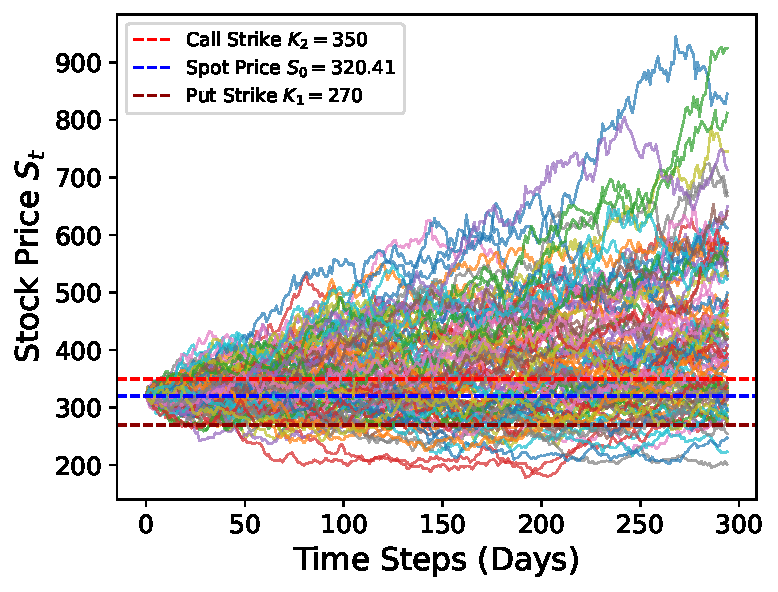
\includegraphics[width=0.5\linewidth]{pppn_simulated_paths.pdf}
    \caption{\textbf{Simulation.} 100 of the $10^4$ simulated paths of \gls{jpm} over 294 trading days. The horizontal lines mark the strikes $K_1$ and $K_2$ and the spot price $S_0$.}
    \label{fig:jpm-simulation}
\end{figure}

Fig.~\ref{fig:jpm-simulation} shows a sample of the paths.
Over $10^4$ paths, the stock leaves the corridor in $76.9\%$ of the cases, and the expected premium at maturity and its present value are
\[
    \hat{\mathbb{E}}[\text{Premium}(S_T)] = 95.57, \qquad e^{-rT}\, \hat{\mathbb{E}}[\text{Premium}(S_T)] = 91.60 > 41.54 = EP(K_1, T) + EC(K_2, T).
\]
The gap does not mean the options are cheap. It comes from the historical drift of \gls{jpm}, which is far above the risk-free rate.
The expected total payoff is
\[
    0.9N + \hat{\mathbb{E}}[\text{Premium}(S_T)] = 288.37 + 95.57 = 383.94,
\]
which corresponds to a growth factor of $\frac{383.94}{S_0} \approx 1.198$, or about $20\%$ on the initial investment.
